
\chapter{Konzept}
\label{sec:konzept}
Dieses Kapitel spezifiziert die umzusetzenden Testfälle. Diese beinhalten die Ausführung, die erwarteten Resultate sowie allfällige Nachbedingungen. Die Vorbedingungen sind für alle Testfälle gleich, da jeder in einer neuen virtuellen Maschine (siehe \Gls{glos:virtualMachine}) gestartet wird und somit keine \Glspl{glos:session} und \Glspl{glos:httpcookie} vorhanden sind.

Um die Kosten zu minimieren werden möglichst wenig Testfälle spezifiziert, jedoch trotzdem die gesamte Funktionalität der Webseite überprüft werden kann. Weitere Details dazu sind im \cref{sec:analyse} \nameref{sec:analyse} aufgeführt.

Eine Übersicht der Testfälle wurde im Wiki von Hotelplan erstellt und wird zum Verständnis dort gepflegt. Die Liste ist im \cref{app:Testfälle} \nameref{app:Testfälle} unter "`Test Cases"' beigefügt.

\section{Übersicht}
Die Seite der travelwindow AG besteht aus drei Bereichen (auch Engines genannt):
\begin{itemize}
\item Citytrip (Flug \& Hotel)
\item Flug
\item Hotel
\end{itemize}

Die Tests werden in drei Kategorien unterteilt:
\begin{itemize}
\item Happy Path
\item Smoke Tests
\item Main Tests
\end{itemize}

Bei den Happy Path Tests wird der gesamte Such- und Buchungungsprozess pro Engine einmal durchlaufen, ohne eine Auswahl zu treffen, oder auf Fehler zu überprüfen. Der Test ist erfolgreich, wenn die letzte Seite des Buchungsprozesses erreicht werden kann. Damit wird sichergestellt, dass die Webseite im Standartdurchlauf keine Fehler produziert.

Die Smoke Tests führen eine Suche für die in der \cref{sec:Recherche:Zielgruppe:top10} \nameref{sec:Recherche:Zielgruppe:top10} definierten Destinationen aus und überprüfen, ob Resultate geliefert werden.

Main Tests überprüfen schlussendlich die Funktionalität gemäss den Funktionalitäten im \cref{app:Funktionalitäten} \nameref{app:Funktionalitäten}).

\subsection{Reihenfolge der Tests}
Die wichtigsten Kriterien für eine Buchungsplattform sind folgende:
\begin{itemize}
\item Kunde kann buchen
\item Kunde kann suchen
\item Rest der Funktionalitäten
\end{itemize}
Punkt eins wird von den Happy Path Tests überprüft. Sie versuchen auf dem direktesten Weg eine Buchung abzuschliessen. Als zweites werden die Smoke Tests durchgeführt, da sie testen ob ein Kunde für die Top 10 Destinationen Resultate finden kann. Schlussendlich werden die Main Tests gestartet um den Rest der Webseite zu testen.

Innerhalb einer dieser drei Testkategorien wird keine weitere Reihenfolge eingehalten.

\subsection{Kunde \& Passagierangaben}
\label{sec:Konzept:Übersicht:Angaben}
Im Buchungsprozess müssen die Kunden- und Passagierangaben ausgefüllt werden. Für alle Tests werden folgenden Daten verwendet:\\
\\  
Kundendaten:
\begin{itemize}
\item Vorname: Han
\item Name: Sola
\item Strasse \& Nummer: Bederstrasse 66
\item Postleitzahl: 8002
\item Ort: Zürich
\item E-Mail Adresse: info@travel.ch
\item Telefonnummer: +41 44 200 26 26 
\end{itemize}

\begin{addmargin*}[0cm]{0\marginwidth}
Passagierangaben (Geschlecht, Vorname, Name, Geburtsdatum):
	\begin{itemize}
	\item Passagier 1: Männlich, Han, Solo, 24.03.1980
	\item Passagier 2: Weiblich, Leia Organa, Solo, 12.02.1978
	\item Passagier 3: Männlich, Luke, Skywalker, 07.08.1985
	\end{itemize}
\end{addmargin*}


\subsection{Datumsangaben}
Die möglichen Eingabewerte für die Reisedaten sind im \cref{sec:analyse:grenzwertanalyse} \nameref{sec:analyse:grenzwertanalyse} beschrieben.
Gemäss der Priorisierung der Funktionalität (siehe  \cref{sec:analyse:testabdeckung} \nameref{sec:analyse:testabdeckung}) werden die Grenzwerte der Reisedaten nicht im Umfang dieses Projektes getestet. Deshalb werden fix folgende Daten verwendet:

\begin{itemize}
\item Startdatum: 3 Monate in die Zukunft, erster Tag des Monats.
\item Enddatum: 3 Monate in die Zukunft, dritter Tag des Monats.
\end{itemize}
\vspace{0 mm}
Die obigen Reisedaten sind dynamisch angegeben, da keine fixen Werte definiert werden können. Ansonsten würde spätestens in einem Jahr, wenn das fixe Datum überschritten wurde, die Tests fehlschlagen.

\section{Happy Path}
Der Happy Path testet, ob beim Standard Szenario keine Fehler auftreten. Jede Engine wird einmal durchlaufen und es werden nur gültige Eingaben vorgenommen. Dies soll überprüfen, ob keine grundlegenden Fehler vorhanden sind.

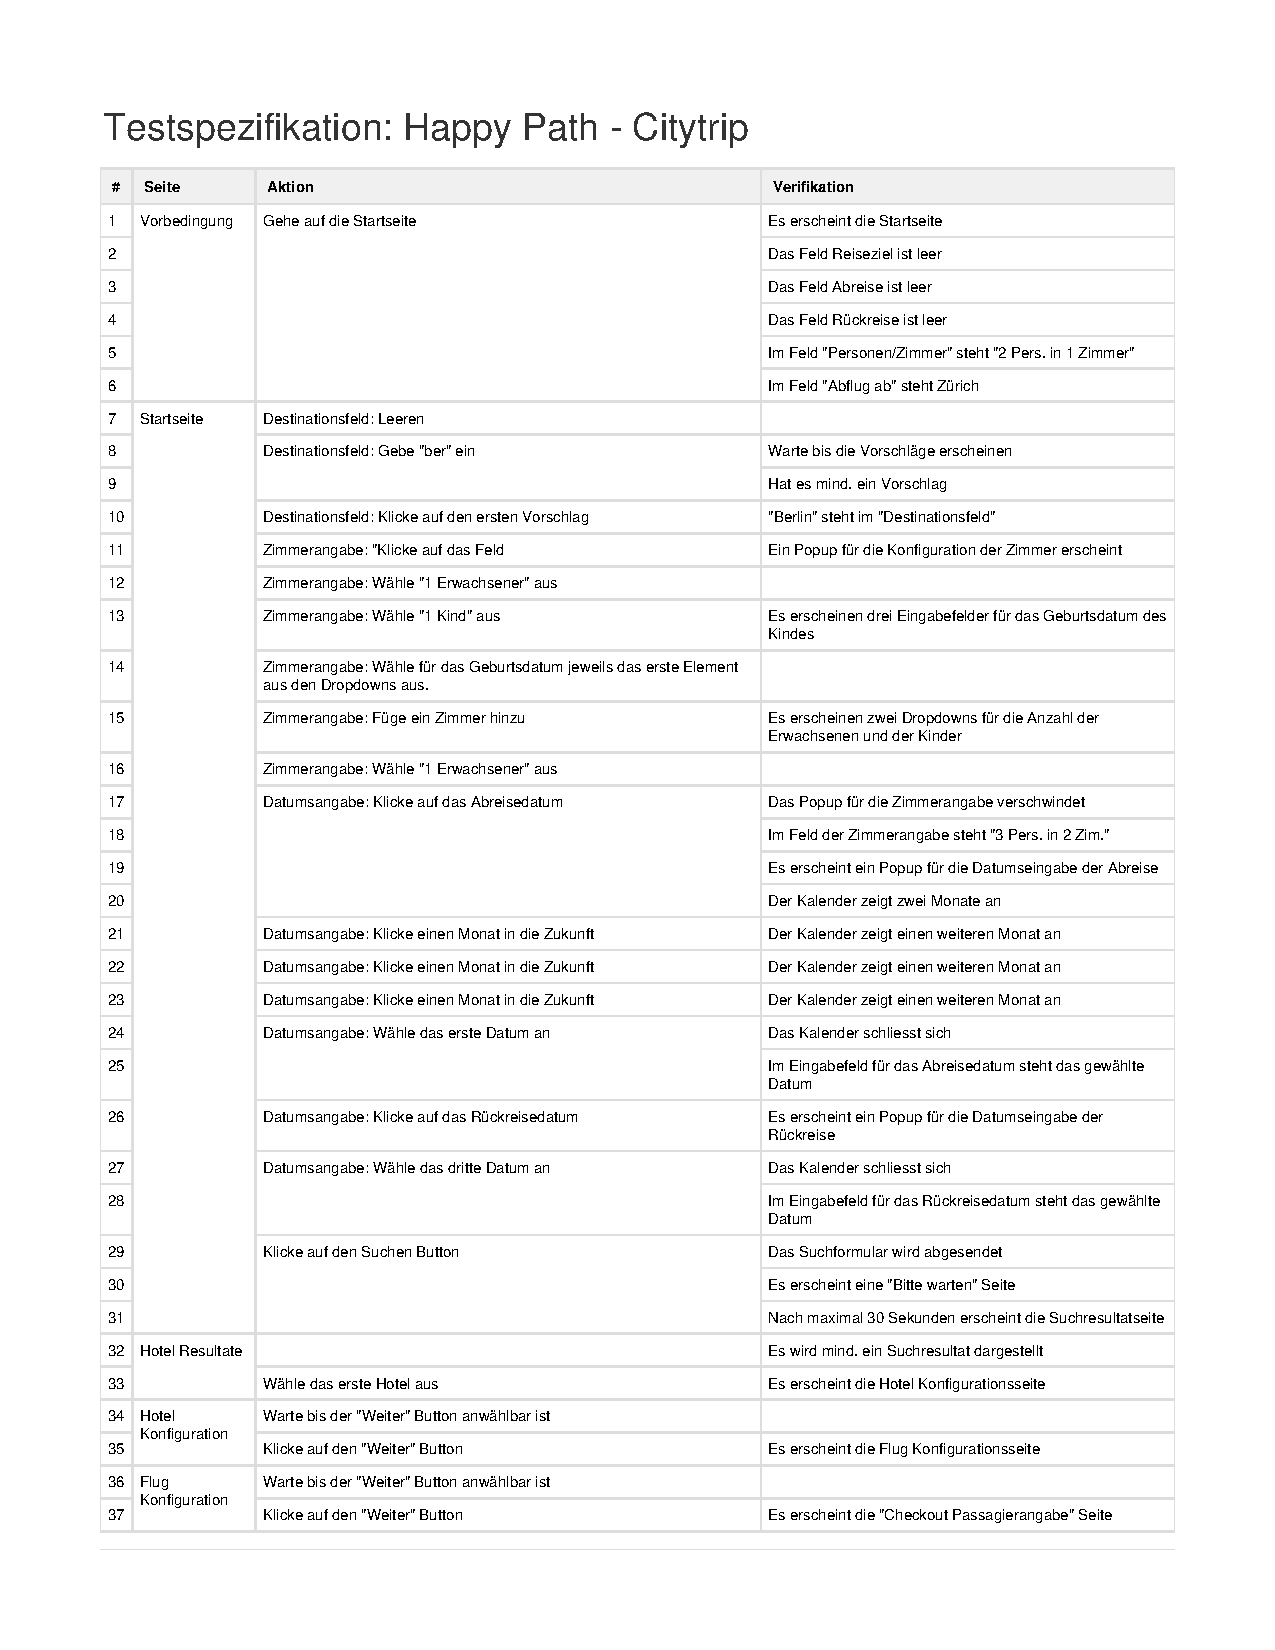
\includepdf[scale=0.8,pages=1,pagecommand=\subsection{Citytrip}]{./../Testspezifikation: Happy Path - Citytrip.pdf}
\includepdf[scale=0.8,pages=2,pagecommand=\subsubsection{}]{./../Testspezifikation: Happy Path - Citytrip.pdf}

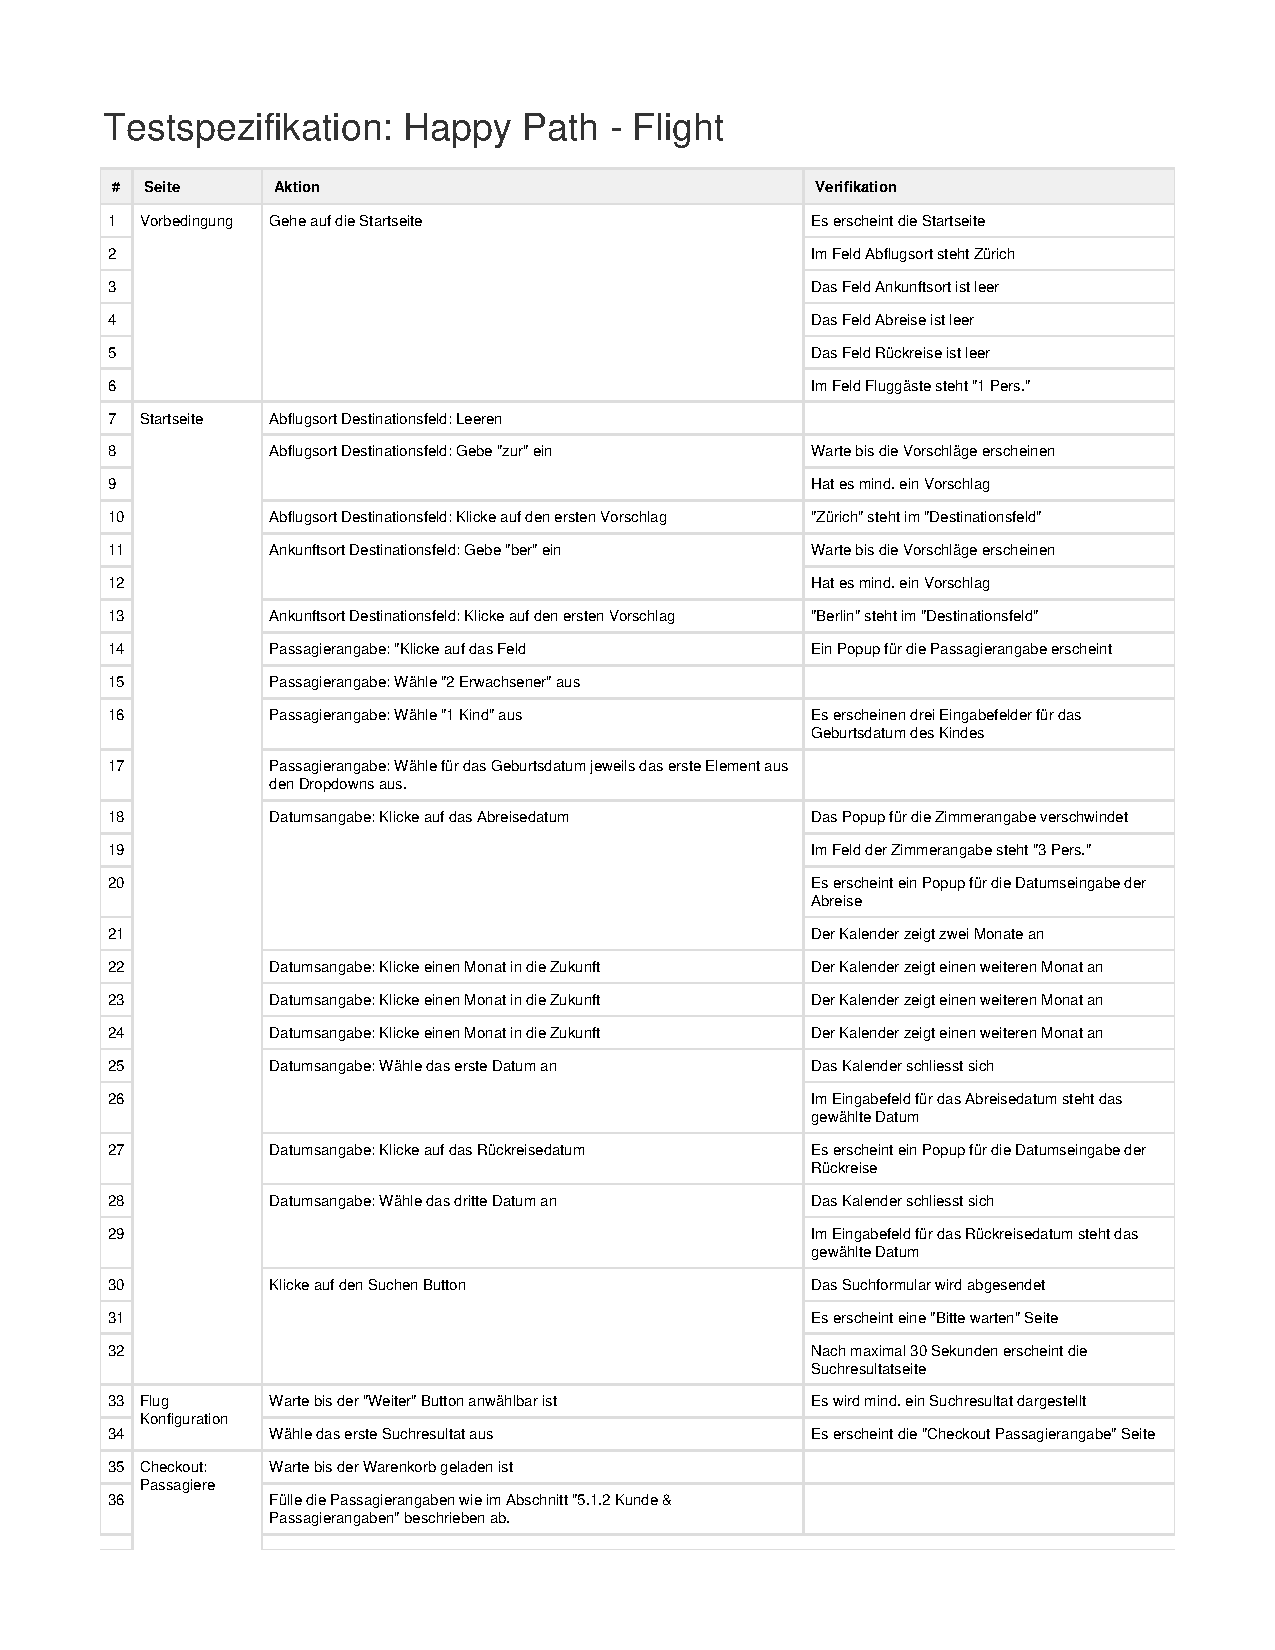
\includepdf[scale=0.8,pages=1,pagecommand=\subsection{Flight}]{./../Testspezifikation: Happy Path - Flight.pdf}
\includepdf[scale=0.8,pages=2,pagecommand=\subsubsection{}]{./../Testspezifikation: Happy Path - Flight.pdf}

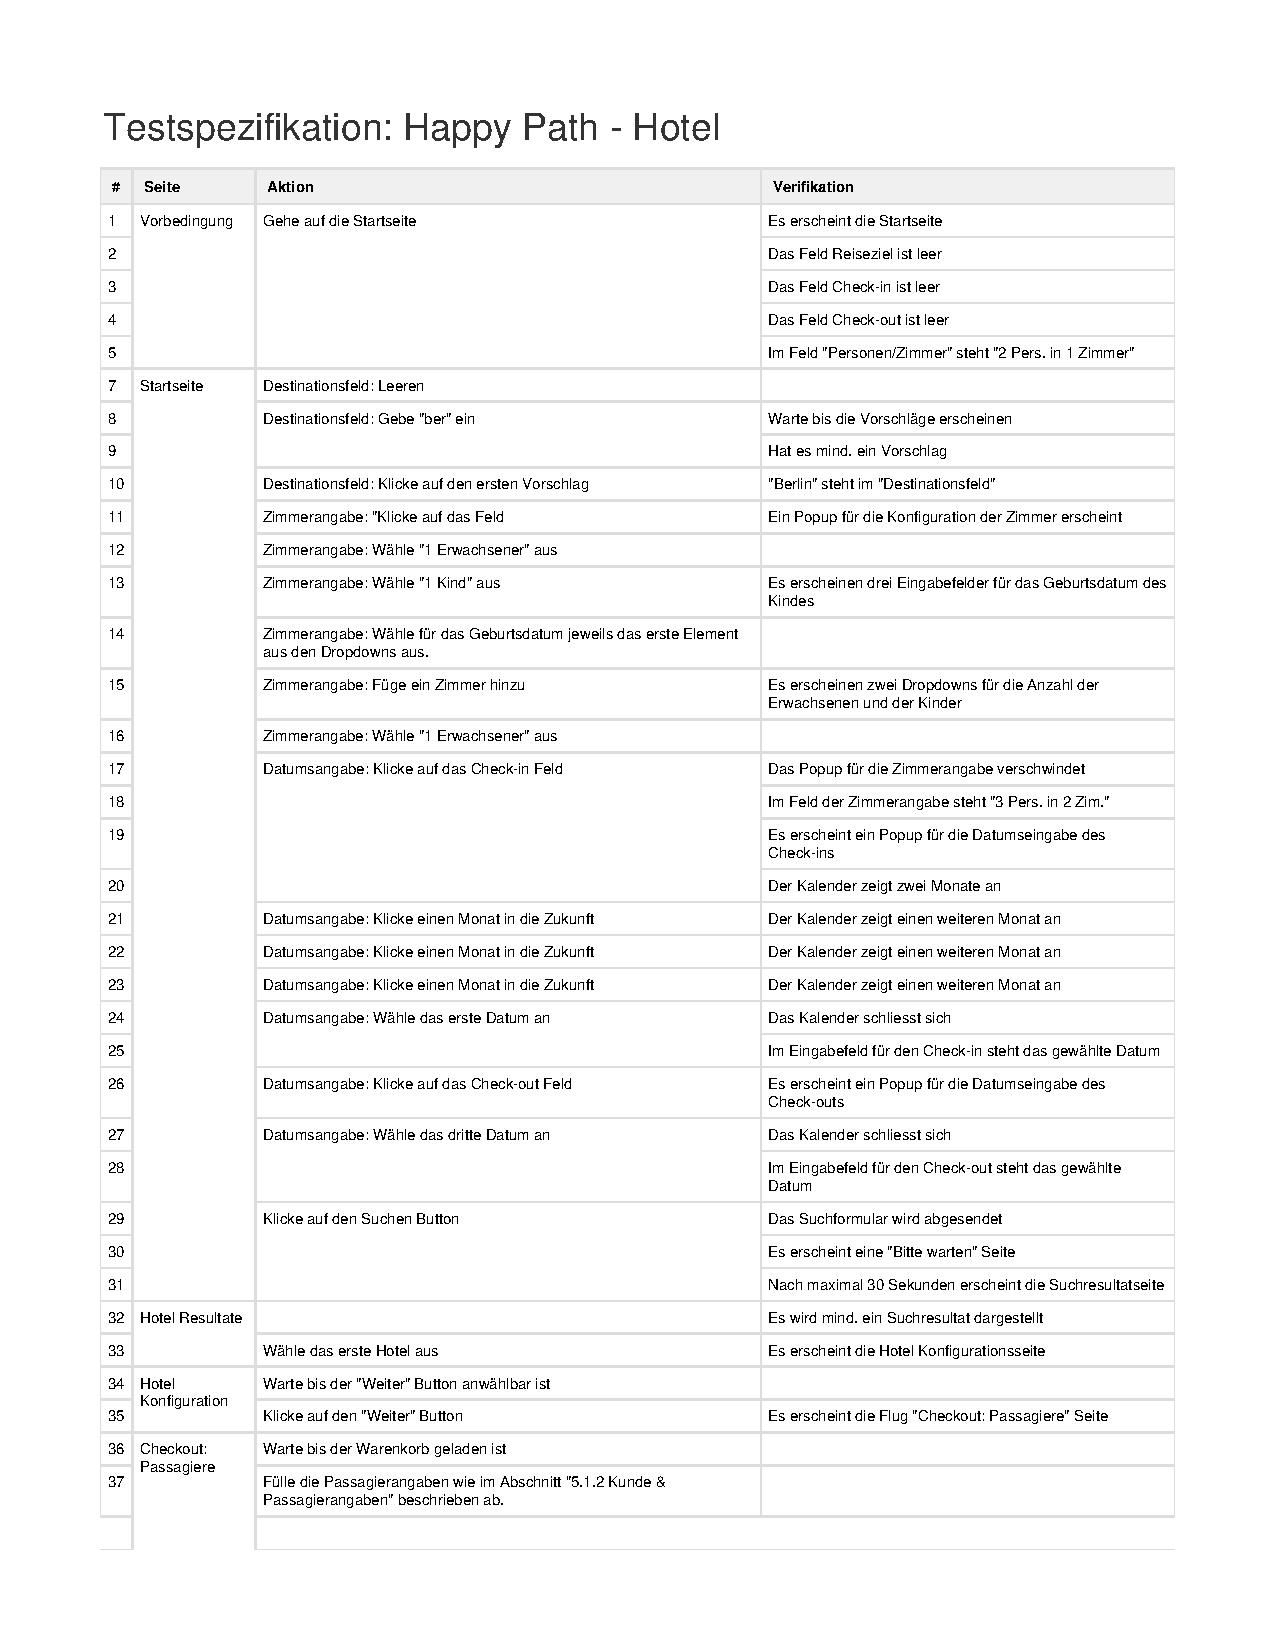
\includepdf[scale=0.8,pages=1,pagecommand=\subsection{Hotel}]{./../Testspezifikation: Happy Path - Hotel.pdf}
\includepdf[scale=0.8,pages=2,pagecommand=\subsubsection{}]{./../Testspezifikation: Happy Path - Hotel.pdf}


\section{Smoke Tests}
\label{sec:konzept:smoketests}
Smoke Tests führen eine Aktion durch und schauen lediglich, ob kein Fehler aufgetreten ist. Der Begriff rührt daher, dass eine Maschine gestartet und getestet wurde, ob sie nicht beginnt zu rauchen\footcite{Smoke_testing_software_-_Wikipedia_the_free_encyclopedia_2015-08-01}.

Bei den folgenden Smoke Tests werden pro Engine die jeweiligen Top 10 (siehe \cref{sec:Recherche:Zielgruppe:top10} \nameref{sec:Recherche:Zielgruppe:top10}) Destinationen gesucht und überprüft, ob Suchresultate geliefert werden.

Die Tests sind pro Engine immer gleich aufgebaut. Die Suchparameter sind dieselben und auch die Verifikation, ob kein Fehler auftraten, ist äquivalent. Das Einzige, was sich unterscheidet, sind die Destinationen. Daher wird jeweils nur der Test für die erste Destination ausführlich spezifiziert. Für die restlichen 9 gilt der selbe Ablauf.

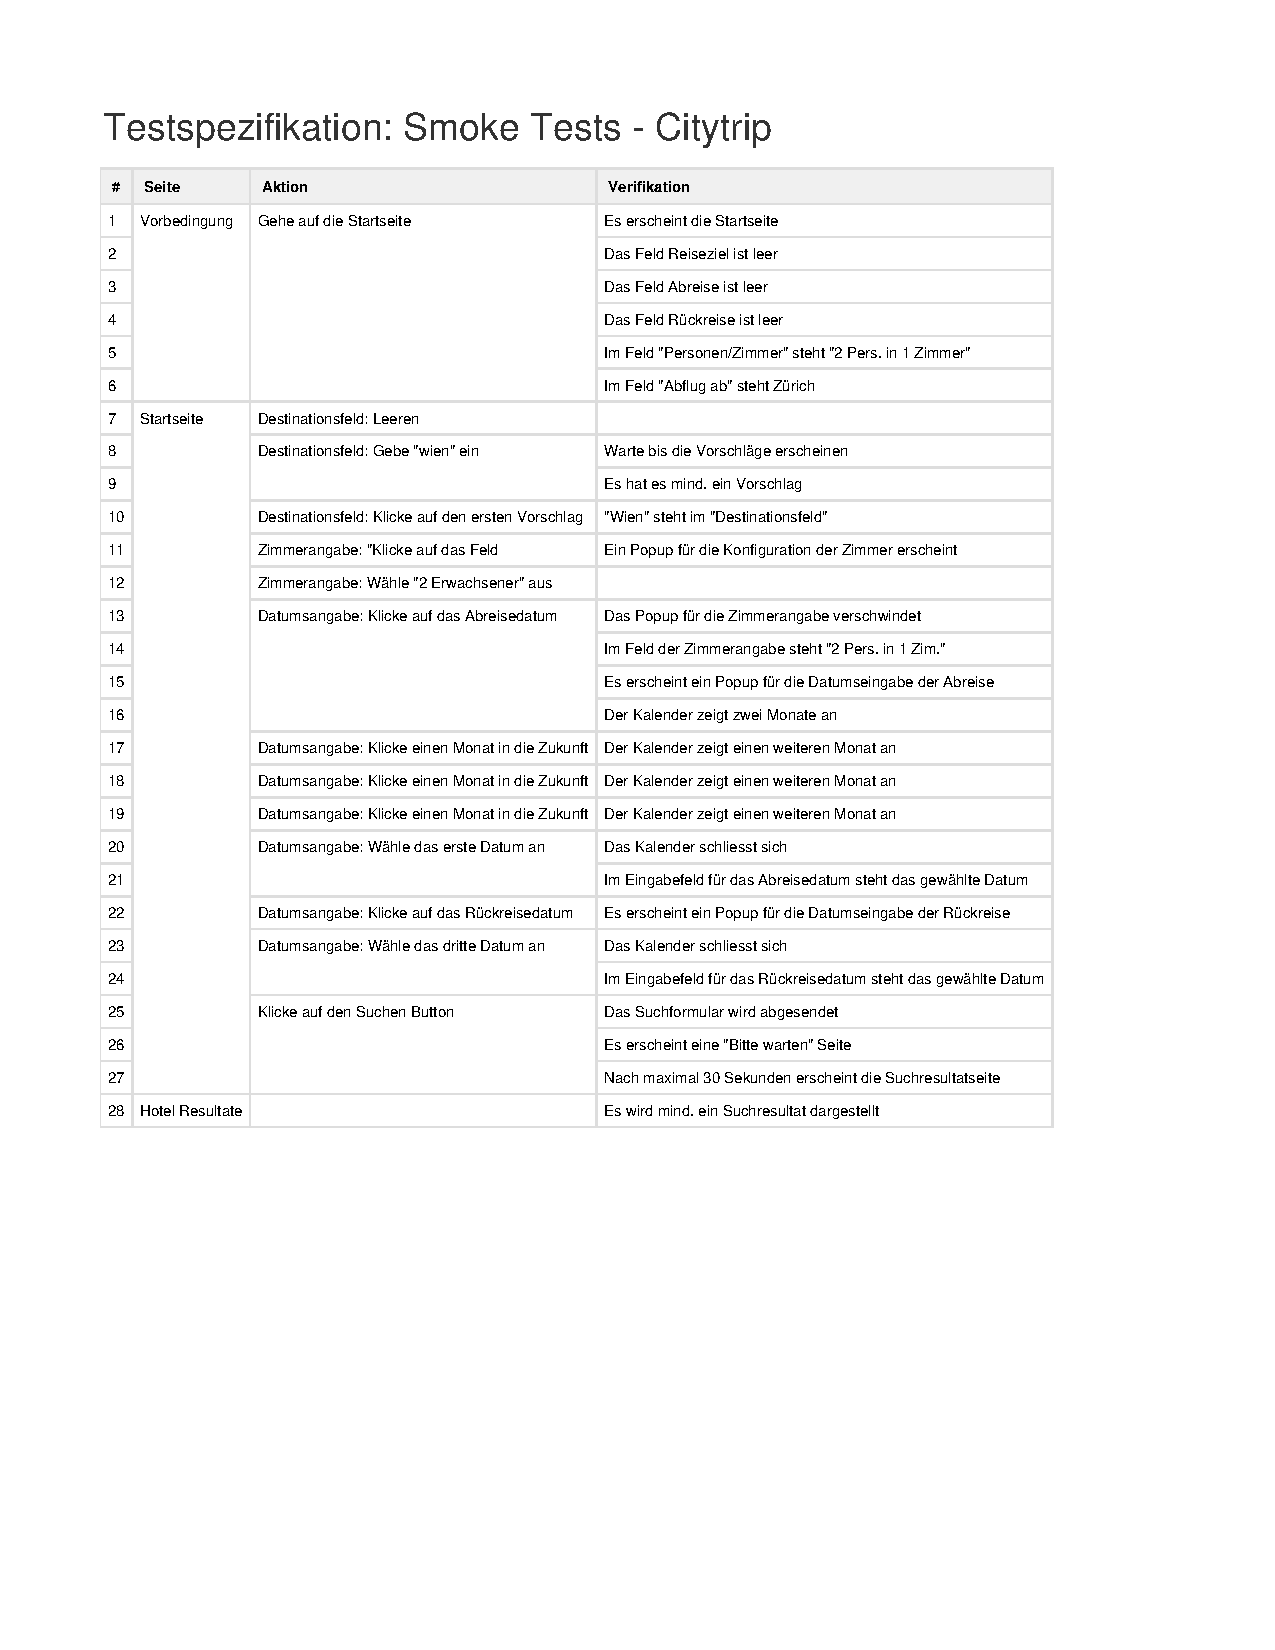
\includepdf[scale=0.8,pages=1,pagecommand=\subsection{Citytrip}]{./../Testspezifikation: Smoke Tests - Citytrip.pdf}

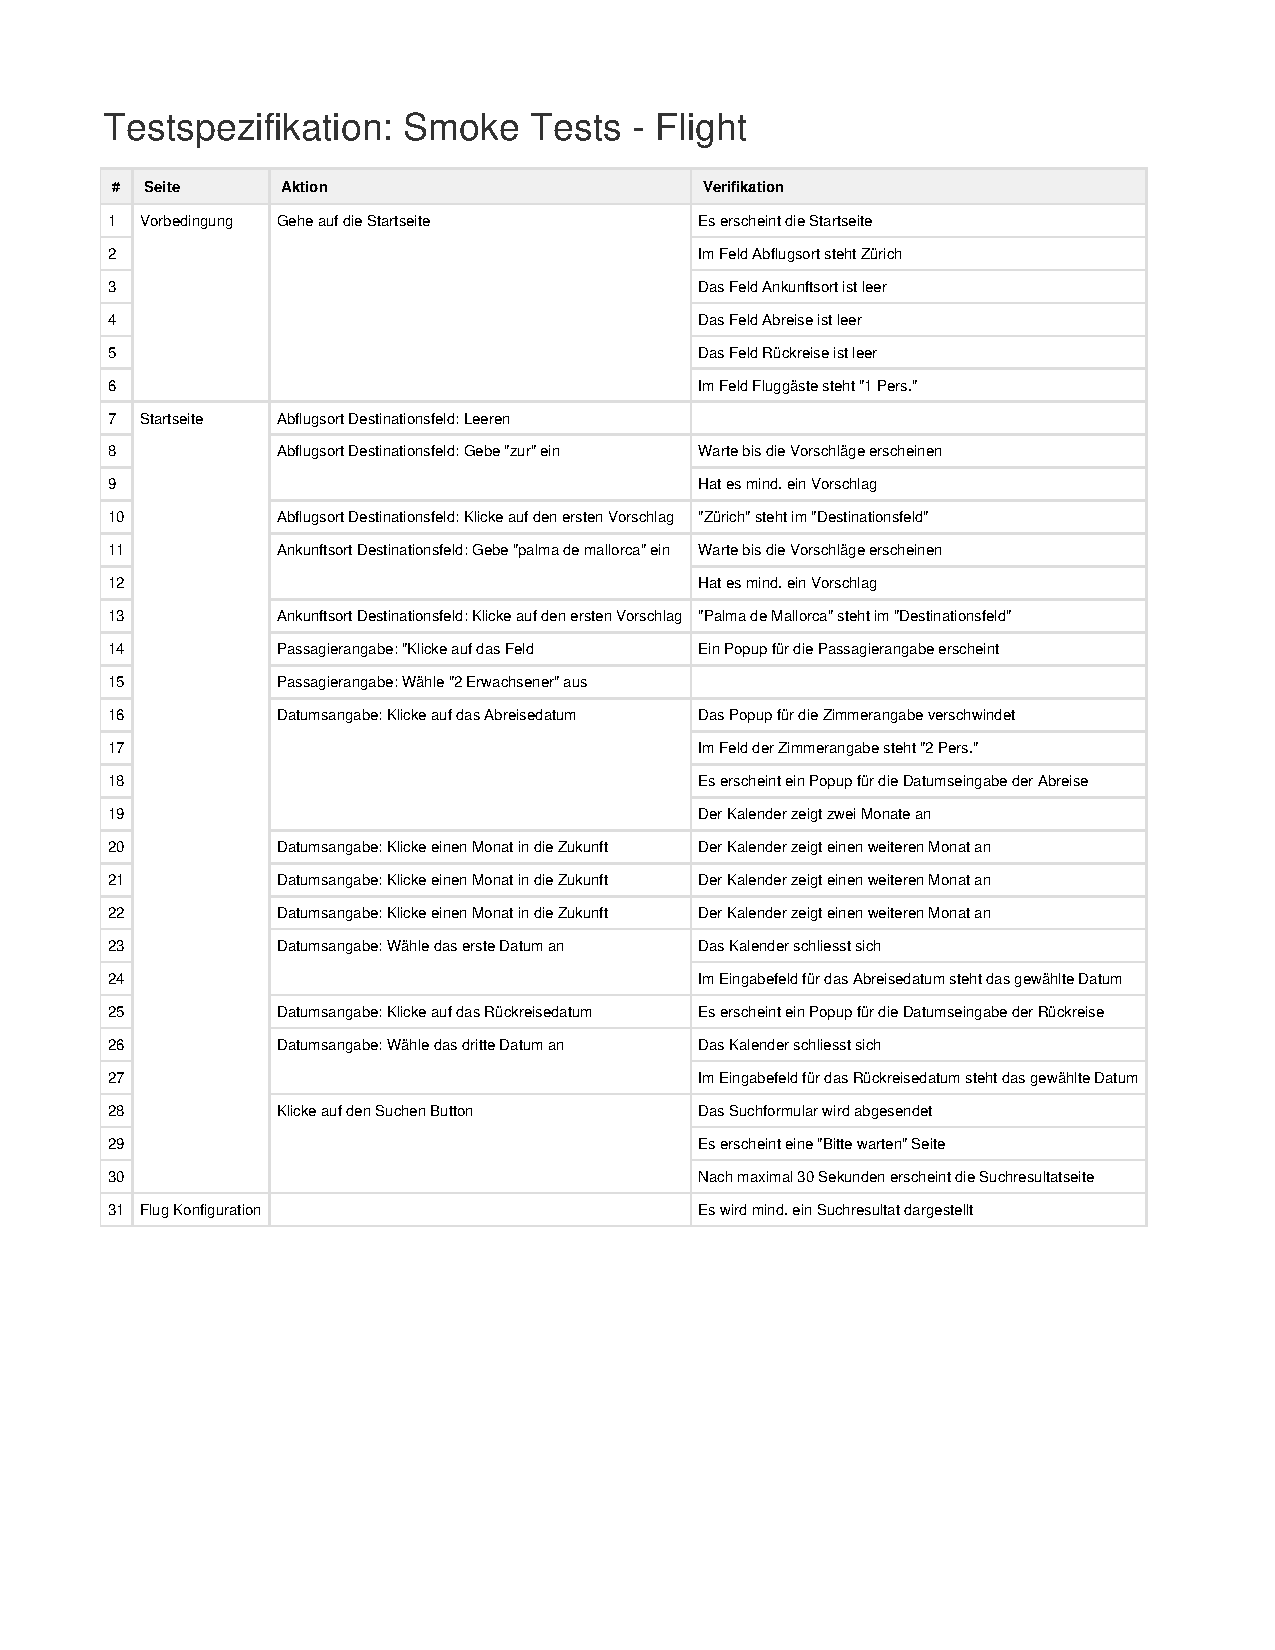
\includepdf[scale=0.8,pages=1,pagecommand=\subsection{Flight}]{./../Testspezifikation: Smoke Tests - Flight.pdf}

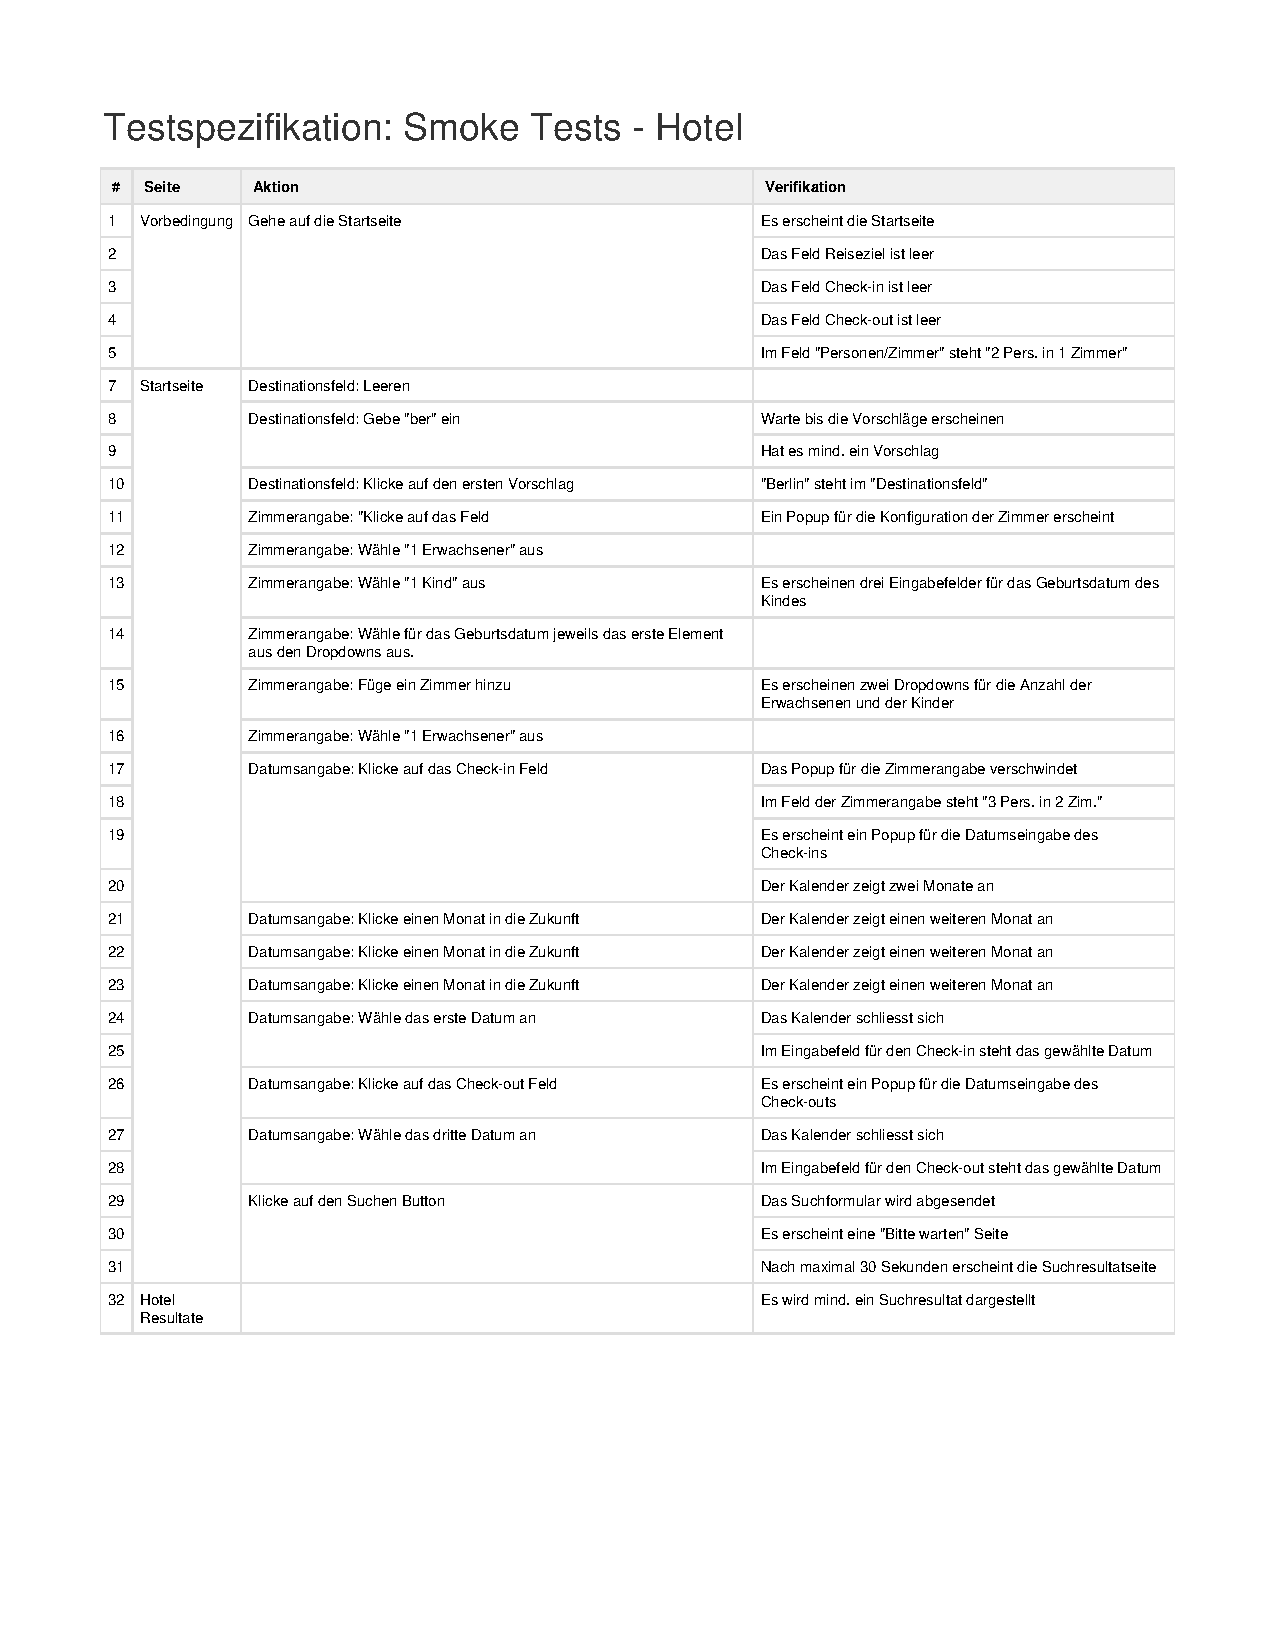
\includepdf[scale=0.8,pages=1,pagecommand=\subsection{Hotel}]{./../Testspezifikation: Smoke Tests - Hotel.pdf}

\section{Main Tests}
Bei den Happy Paths wird überprüft, ob die Funktionalität der Webseite gemäss Spezifikation (siehe \cref{app:Funktionalitäten} \nameref{app:Funktionalitäten}) umgesetzt wurde. Die Funktionalitäten im Anhang sind priorisieriert und werden gemäss dieser umgesetzt. Begonnen wurde mit der höchsten Zahl.


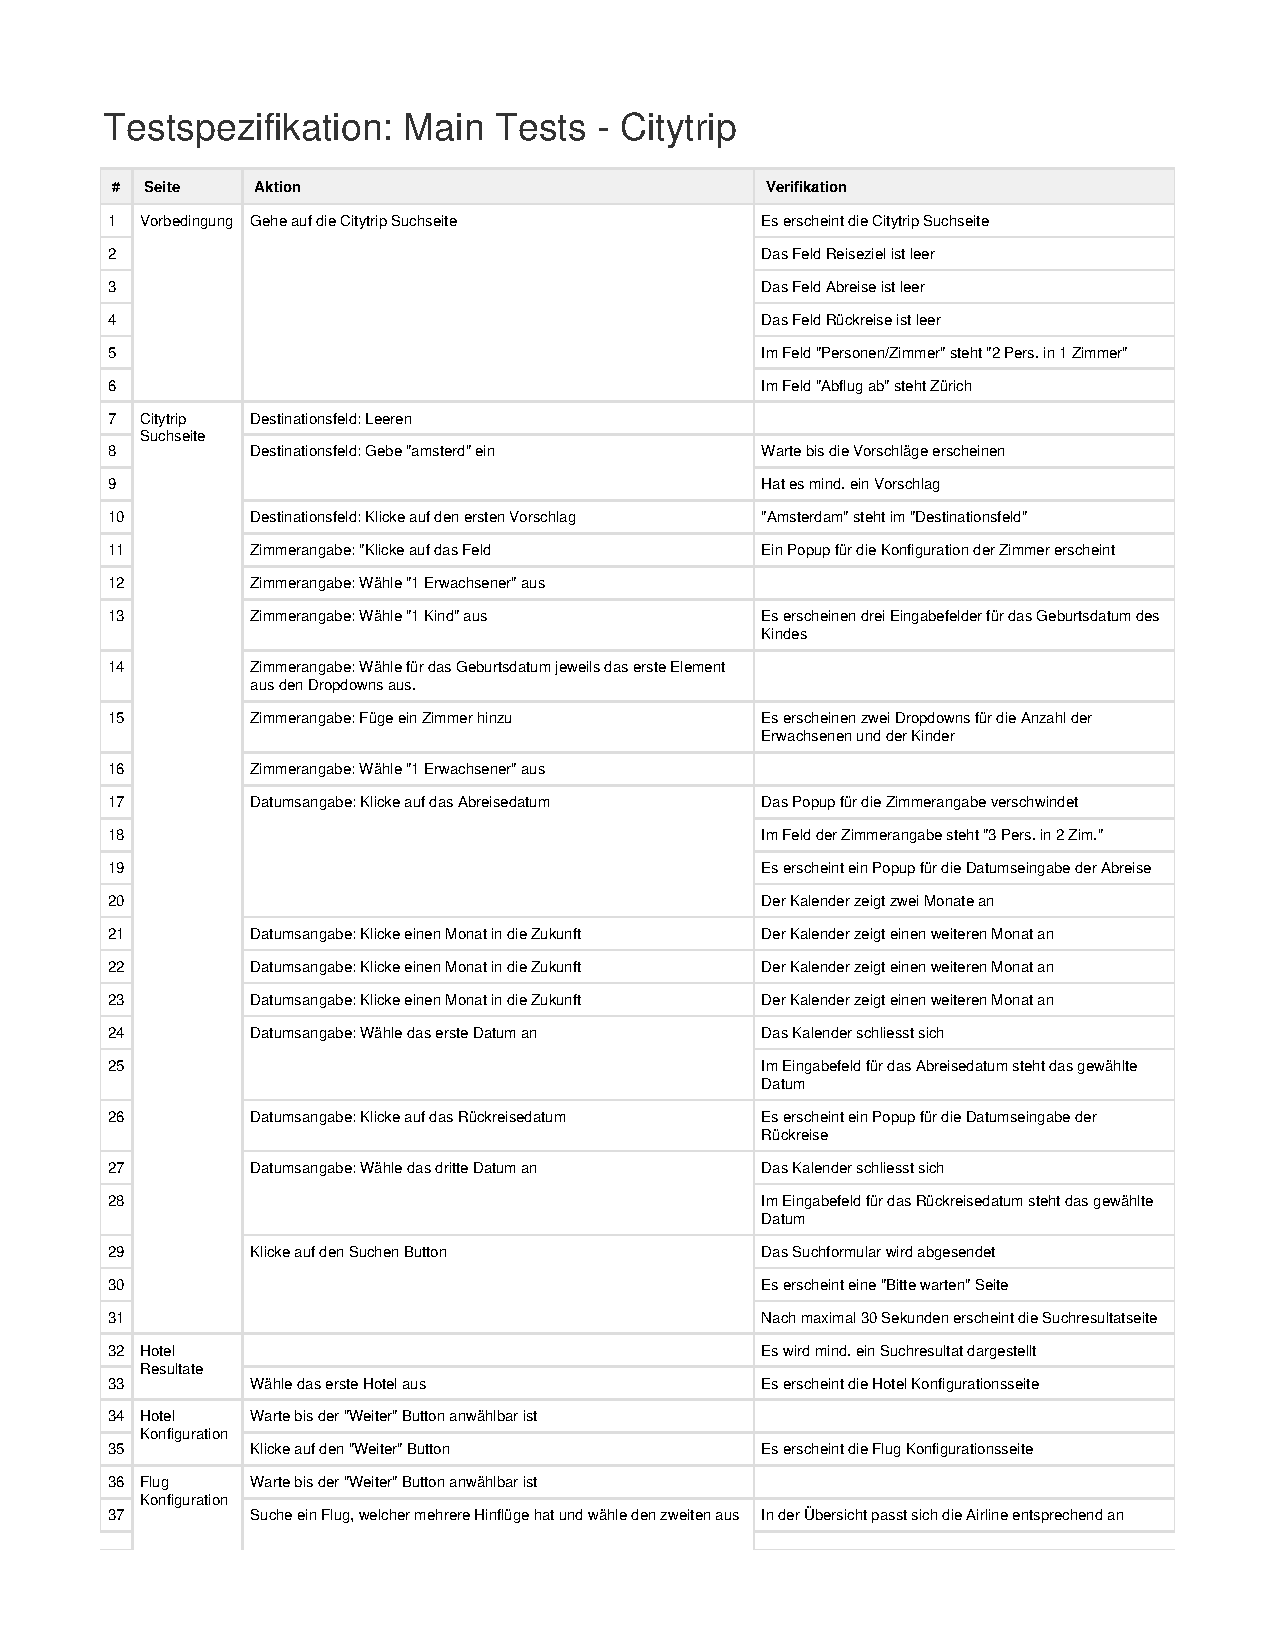
\includepdf[scale=0.8,pages=1,pagecommand=\subsection{Citytrip}]{./../Testspezifikation: Main Tests - Citytrip.pdf}
\includepdf[scale=0.8,pages=2,pagecommand=\subsubsection{}]{./../Testspezifikation: Main Tests - Citytrip.pdf}

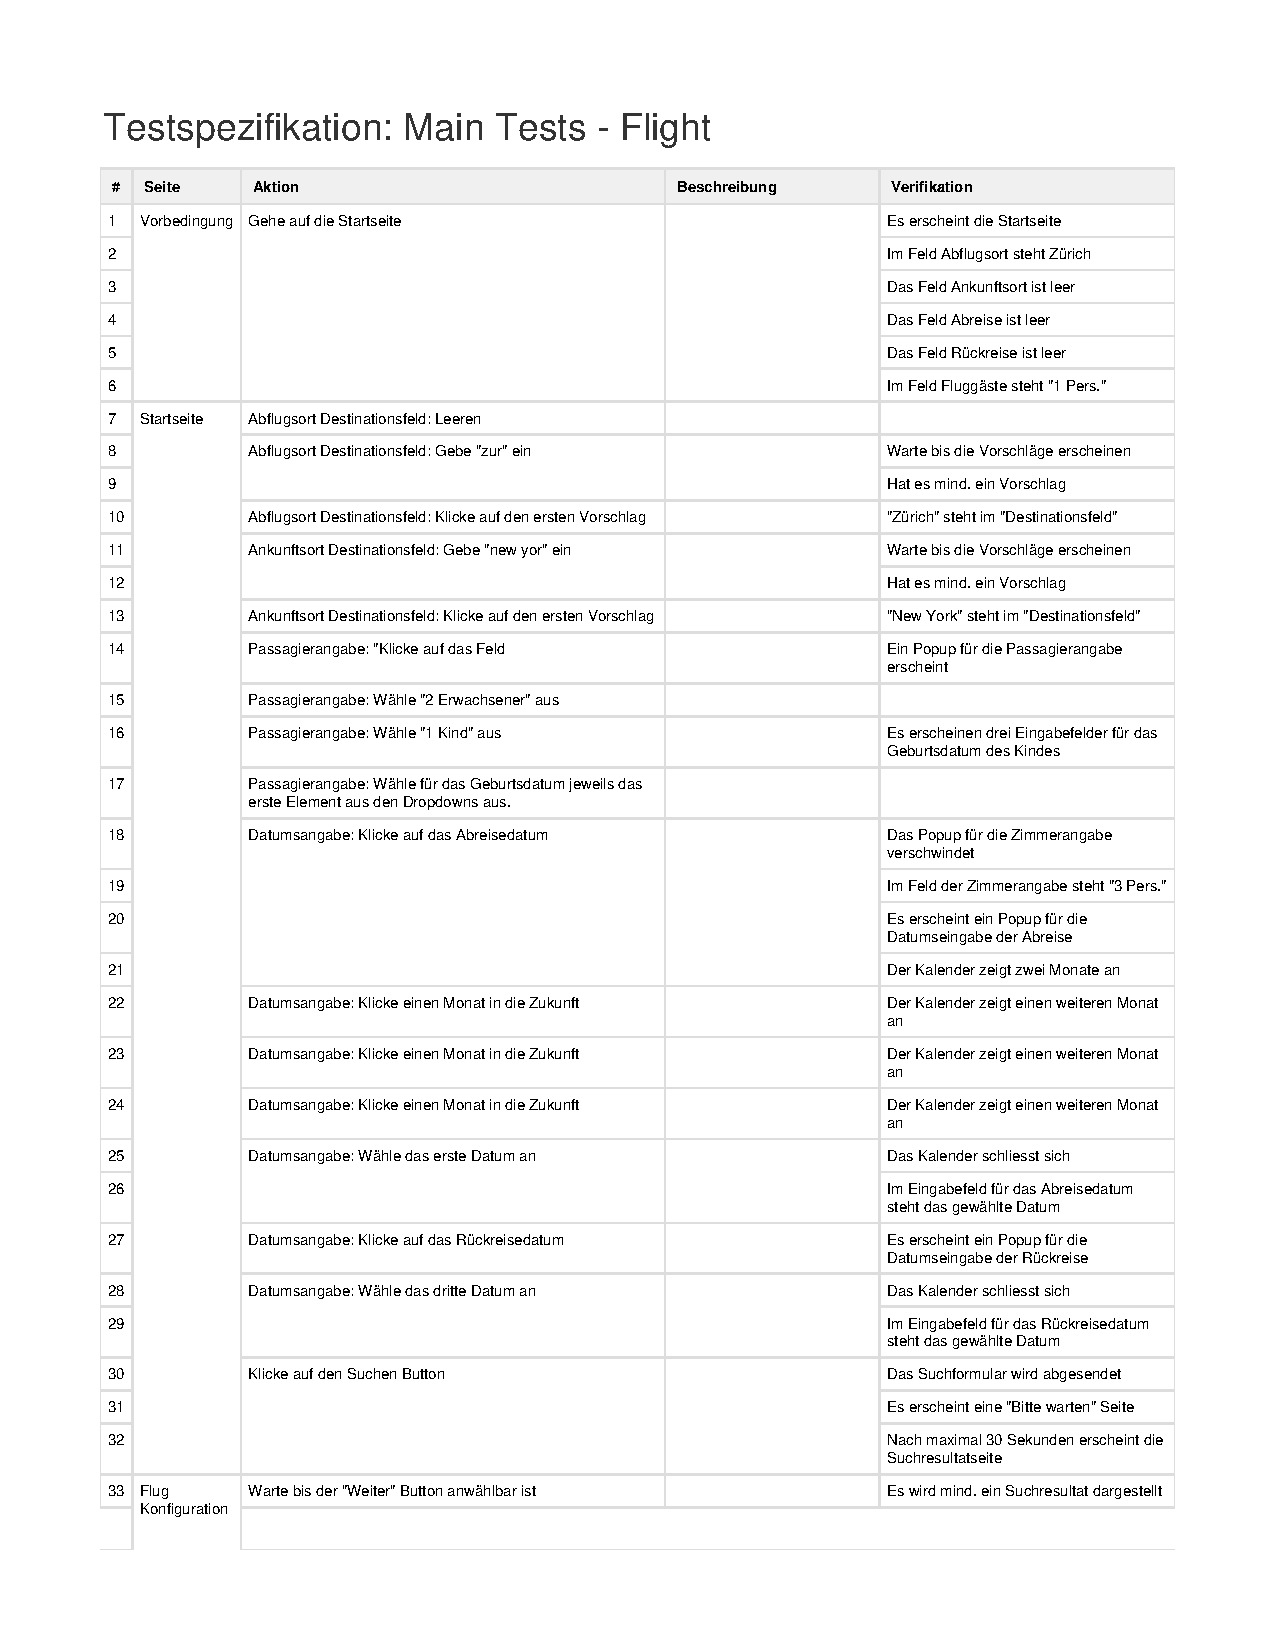
\includepdf[scale=0.8,pages=1,pagecommand=\subsection{Flight}]{./../Testspezifikation: Main Tests - Flight.pdf}
\includepdf[scale=0.8,pages=2,pagecommand=\subsubsection{}]{./../Testspezifikation: Main Tests - Flight.pdf}
\includepdf[scale=0.8,pages=3,pagecommand=\subsubsection{}]{./../Testspezifikation: Main Tests - Flight.pdf}